%!TEX root = ../nwoods_thesis.tex

\chapter{Analysis Strategy}

\section{Background Estimation}
Reducible backgrounds for four-lepton events typically have two prompt leptons and two other objects---typically jet fragments---which are misidentified as prompt leptons.
The largest source of background events, often referred to as ``\PZ+X,'' arises when a {\PZ} boson is produced in association with a leptonically-decaying $\PW$ boson and a jet, or two jets.
There is also a contribution from $\Pqt\Paqt$ events in which both top quarks decay to a lepton, a neutrino, and a {\Pqb}~quark jet.
For simplicity, the two sets of processes are not treated separately in what follows, and are collectively labeled ``\PZ+X'' in the plots.

The contributions of the reducible backgrounds to the selected four-lepton signal samples are evaluated using the tight-to-loose ``fake rates'' method.
The likelihood of a ``loose'' (fake) candidate to be misidentified as a  ``tight'' (prompt) lepton is estimated and applied to control regions with loose candidates to estimate their contribution to the signal region.
The lepton misidentification rate $f_l\left(\pt, \eta\right)$ is measured from a sample of $\PZ + \ell_\text{loose}$ events, where the {\PZ} candidate is selected as in the signal region but with $\left| m_{\ell\ell} - m_\PZ \right| < 10\GeV$, and the $\ell_\text{loose}$ candidate is a lepton candidate that passes relaxed ID requirements as defined in Section~\ref{sec:looseID}, with no isolation or tight ID requirements applied.

The misidentification rate is defined as the fraction of $\ell_\text{loose}$ candidates which pass full lepton identification and isolation critera, in bins of $\pt$ and $\eta$.
One should note that this is not a probability in the usual sense, and there is not a simple physical interpretation of these misidentification rates.\
Figure~\ref{fig:fakerates} shows the misidentification rates for electrons and muons separately as a function of {\pt} and $\eta$.

%=============
\begin{figure}[htbp]
 \begin{center}
   \subfigure[]{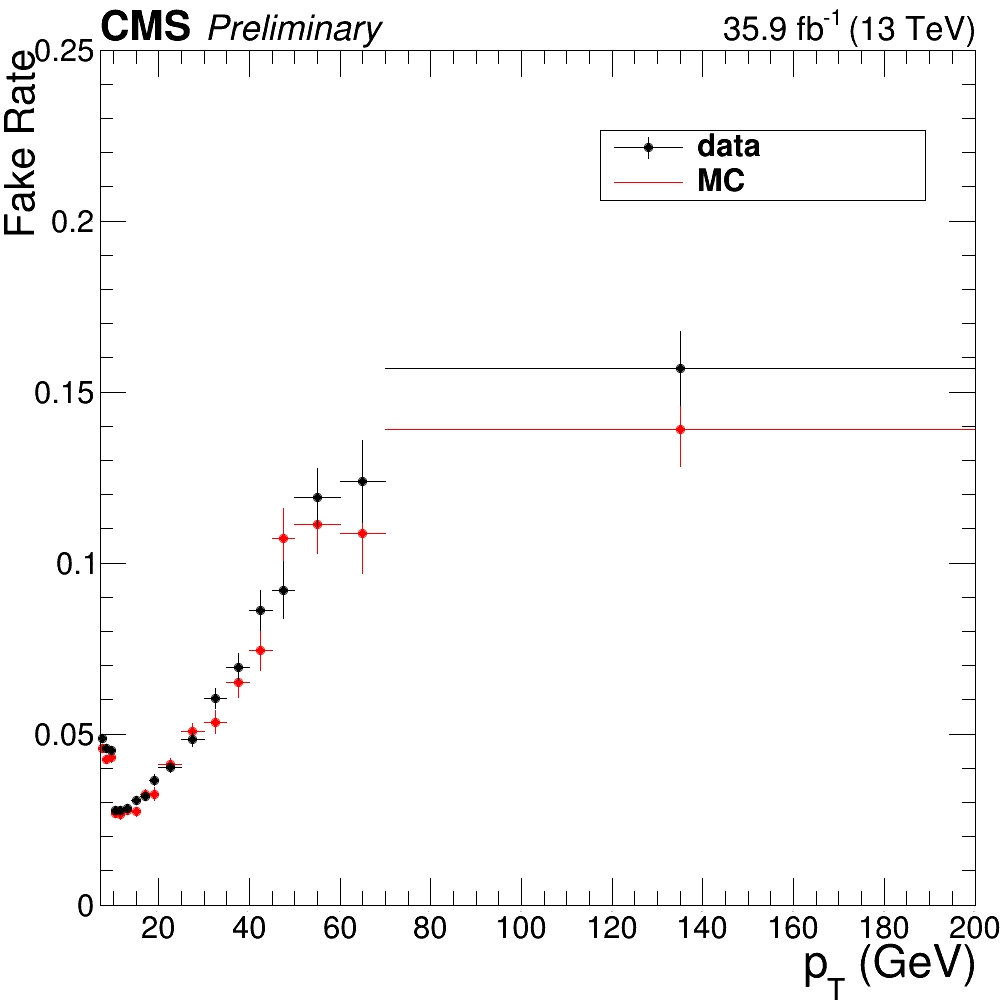
\includegraphics[width=0.35\textwidth]{methods/eFakeRate_pt.png}}
   \subfigure[]{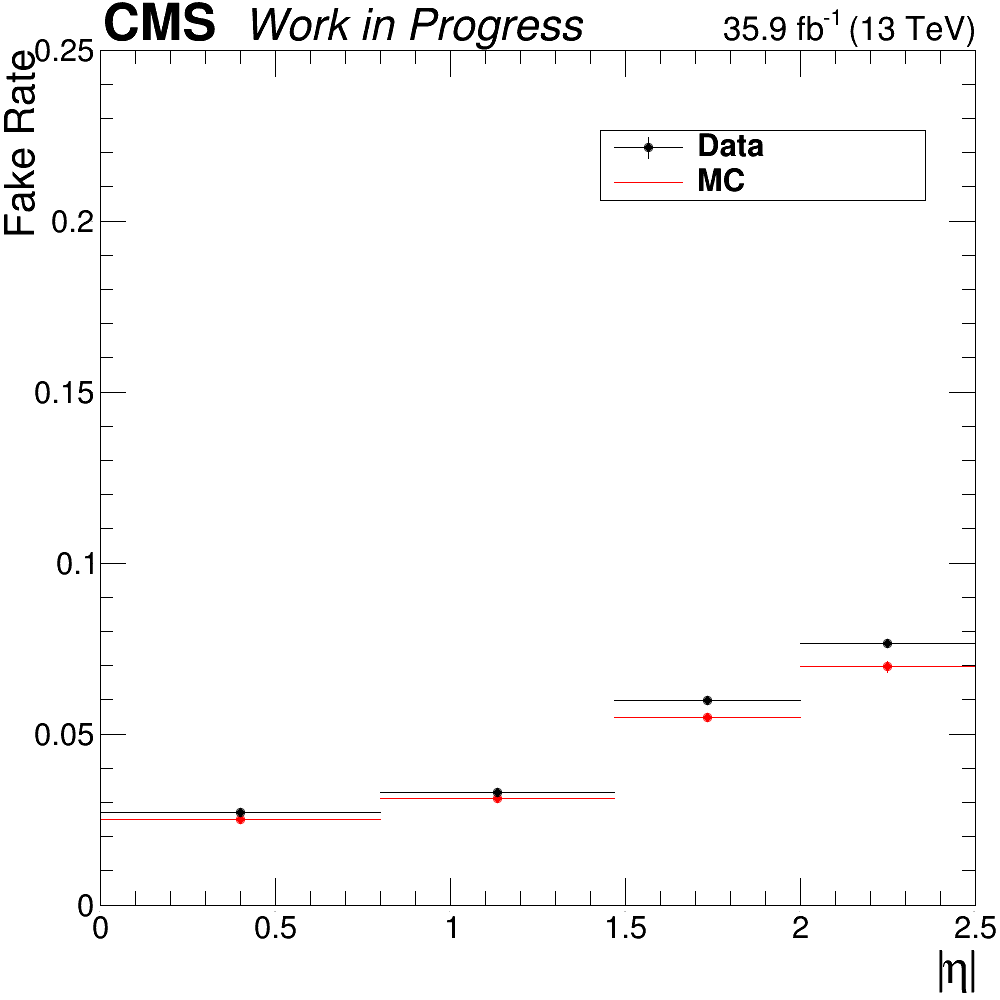
\includegraphics[width=0.35\textwidth]{methods/eFakeRate_eta.png}} \\
   \subfigure[]{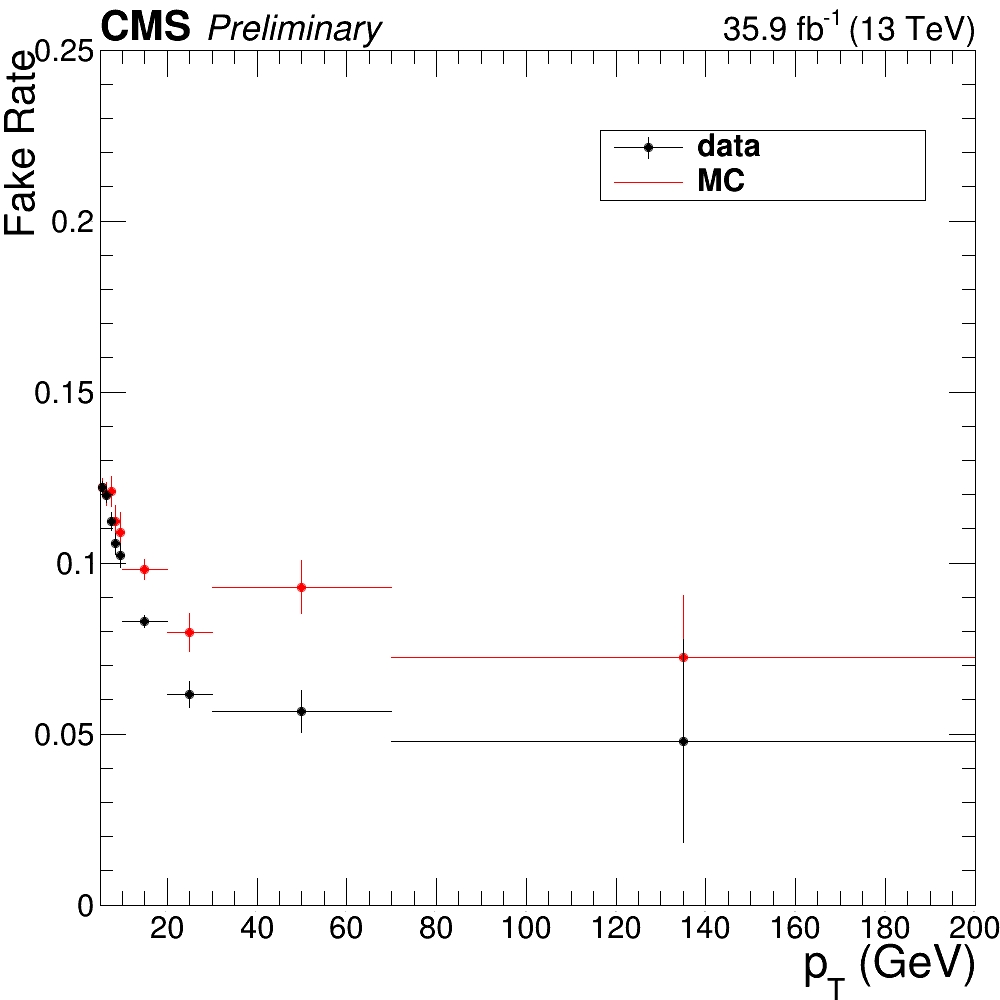
\includegraphics[width=0.35\textwidth]{methods/mFakeRate_pt.png}}
   \subfigure[]{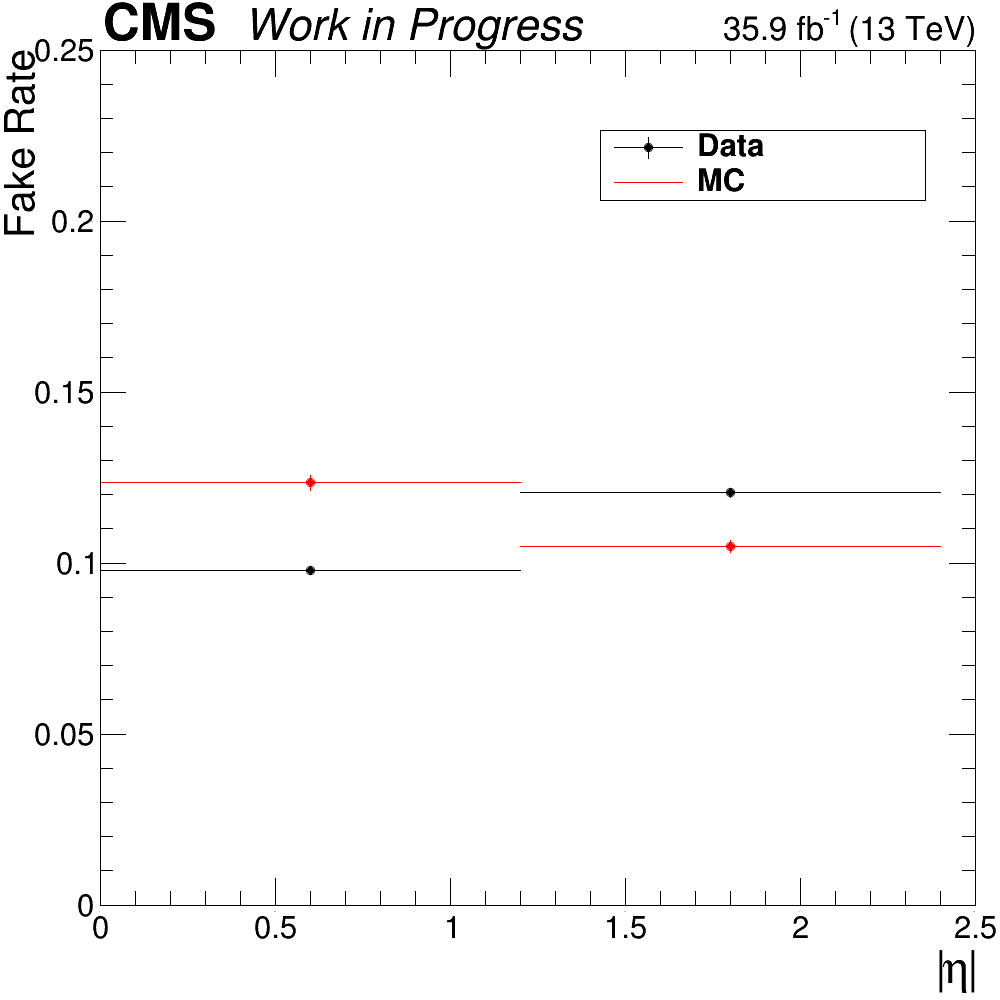
\includegraphics[width=0.35\textwidth]{methods/mFakeRate_eta.png}}
   \caption{
     Fake rate for electron (a,b) and muons (c,d) as a function of $\pt$ and $\eta$.
   }\label{fig:fakerates}
 \end{center}
\end{figure}




\section{Systematic Uncertainties}
Who knows?



\section{Fiducial and Total Cross Section Calculation}

\subsection{Signal Strength Extraction}
Fitting


\subsection{\texorpdfstring{$\mathrm{Z} \to 4\ell$}{Z to 4l} Branching Fraction}
It is tiny



\section{Differential Cross Sections}

\subsection{Unfolding}
IT'S FREQUENTIST\@!


\subsection{Propagation of Systematic Uncertainties}
A small pain



\section{VBS Signal Extraction}
BDTs and other hip things



\section{Anomalous Gauge Coupling Searches}
